%!TEX program = xelatex

\documentclass{cls/simplebeamer}
\usepackage{listings}
\usepackage{graphicx}
\usepackage{subcaption}
\usepackage{tikz}


\begin{document}

\begin{frame}[plain]
  \title{An Example Beamer Presentation}
  \subtitle{CONF 2025}
  \author{林浩 LIN Hao}
  \institute{Dual Technology Institute}
  \date{2025年5月1日}
  \titlepage
\end{frame}

\begin{frame}
  \frametitle{Outline}
  \tableofcontents
\end{frame}

\section{Introduction}

\begin{frame}
  \frametitle{Introduction}
  \begin{itemize}
    \item What is \textcolor{red}{Beamer}?
    \item A \textcolor{structure}{\LaTeX} class for creating presentations.
    \item Advantages:
      \begin{itemize}
        \item Professional look
        \item Easy to create equations
        \item Highly customizable
      \end{itemize}
  \end{itemize}
\end{frame}

\section{中文测试}

\begin{frame}
  \frametitle{中文测试}
  \begin{enumerate}
    \item 用户只需了解基本的 LaTeX 语法,就能快速上手 Beamer。
    \item 通过简单的命令,用户可以插入图像、创建项目符号列表、调整字体样式等,极大地提升了制作效率。
    \item 无论是科研报告、教学课件,还是商务演示,Beamer 都是一个理想的选择。
  \end{enumerate}
\end{frame}

\section{Theorem/Equations}

\begin{frame}
  \frametitle{Theorem}
  \begin{theorem}
    The fibonacci sequence is defined as follows:
    \begin{equation}
      F_n = F_{n-1} + F_{n-2}
    \end{equation}
    where $F_0 = 0$ and $F_1 = 1$.
  \end{theorem}
  \begin{proof}
    The proof is trivial.
  \end{proof}
\end{frame}

\begin{frame}
  \frametitle{Equations}
  
  \begin{equation}
    E = mc^2
  \end{equation}
  \begin{equation}
    \int_0^\infty e^{-x^2} dx = \sqrt{\pi}
  \end{equation}
  \vspace{12pt}
  \begin{equation}
    \begin{aligned}
      \min~ & c^T x \\
      \text{s.t. } & Ax = b\\
      & x \geq 0 
    \end{aligned}
  \end{equation}
\end{frame}

\section{Code/Tables}

\begin{frame}[fragile]
  \frametitle{Code}
  \begin{lstlisting}[language=Python]
  def fib(n):  # fibonacci function
      if n <= 1:
          return n
      else:
          return fib(n-1) + fib(n-2)

  if __name__ == "__main__":
      print(fib(10))
  \end{lstlisting}
\end{frame}

\begin{frame}
  \frametitle{Tables}
  \begin{table}
    \centering
    \caption{学生成绩表}
    \begin{tabular}{|c|c|c|c|c|c|}
        \hline
        \textbf{姓名} & \textbf{数学} & \textbf{语文} & \textbf{英语} & \textbf{物理} & \textbf{化学} \\
        \hline
        张三 & 85 & 78 & 92 & 88 & 90 \\
        \hline
        李四 & 76 & 85 & 80 & 70 & 75 \\
        \hline
        王五 & 90 & 88 & 95 & 92 & 89 \\
        \hline
    \end{tabular}
\end{table}

\begin{table}[h]
  \centering
  \caption{Student Grades Table}
  \begin{tabular}{|c|c|c|c|c|c|}
      \hline
      \textbf{Name} & \textbf{Math} & \textbf{Chinese} & \textbf{English} & \textbf{Physics} & \textbf{Chemistry} \\
      \hline
      Zhang San & 85 & 78 & 92 & 88 & 90 \\
      \hline
      Li Si & 76 & 85 & 80 & 70 & 75 \\
      \hline
      Wang Wu & 90 & 88 & 95 & 92 & 89 \\
      \hline
  \end{tabular}
\end{table}
\end{frame}

\begin{frame}
  \frametitle{Figures}
  \begin{figure}
    \centering
    \begin{subfigure}[b]{0.45\textwidth}
        \centering
        
\includegraphics[width=\textwidth]{previews/simplebeamer1.jpg} % 替换为你的图片文件名
        \caption{Title Page}
        \label{fig:image1}
    \end{subfigure}
    \hfill
    \begin{subfigure}[b]{0.45\textwidth}
        \centering
        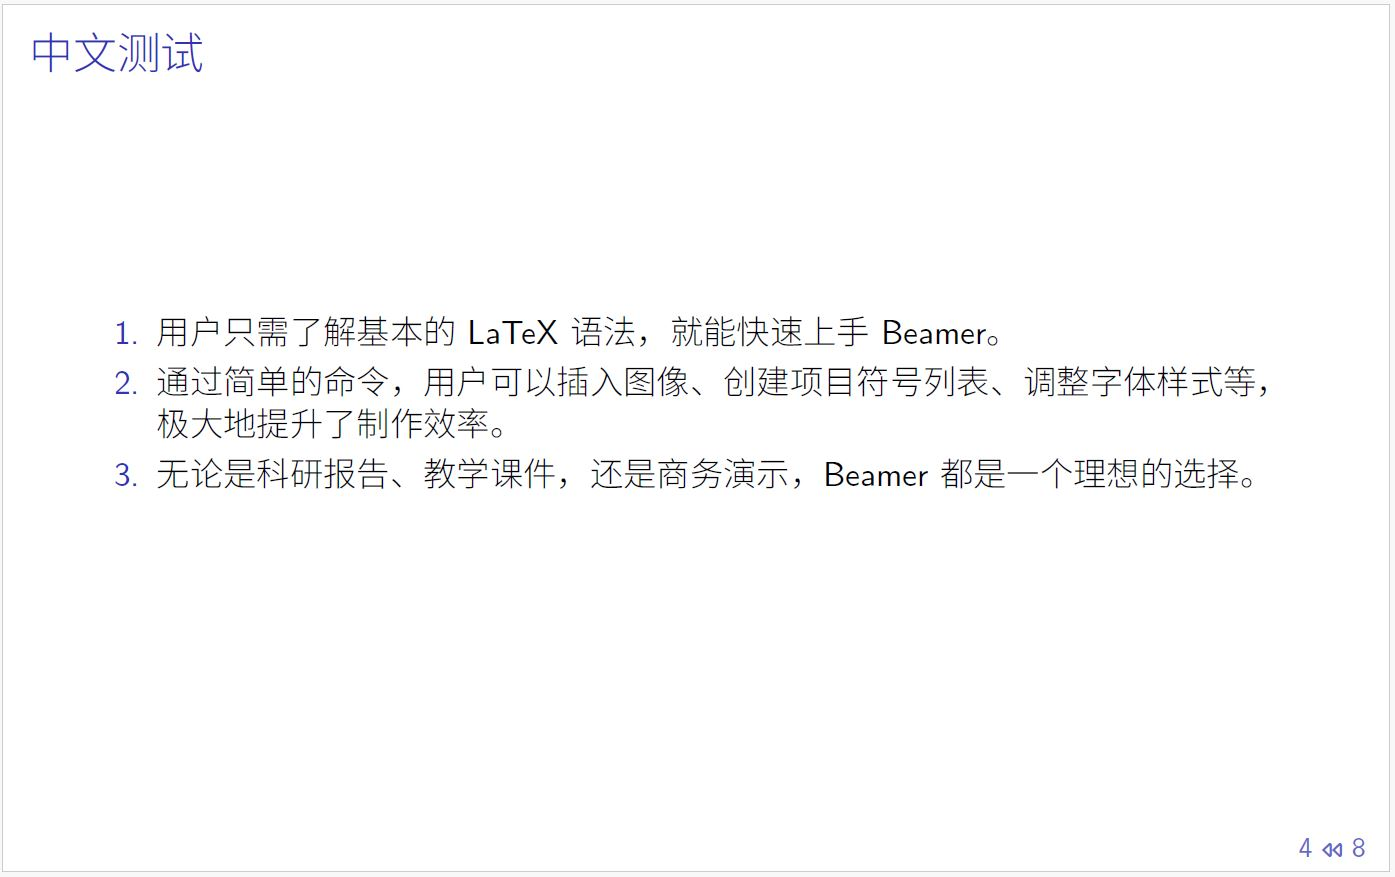
\includegraphics[width=\textwidth]{previews/simplebeamer2.jpg} % 替换为你的图片文件名
        \caption{Frame Page}
        \label{fig:image2}
    \end{subfigure}
    \caption{Simple Beamer Preview}
    \label{fig:two_images}
  \end{figure}
\end{frame}

\begin{frame}
  \frametitle{Tikz}
  \usetikzlibrary{arrows,intersections}
  \centering
  \begin{tikzpicture}[
    thick,
    >=stealth',
    dot/.style = {
      draw,
      fill = white,
      circle,
      inner sep = 0pt,
      minimum size = 4pt
    }
  ]
  \coordinate (O) at (0,0);
  \draw[->] (-0.3,0) -- (8,0) coordinate[label = {below:$x$}] (xmax);
  \draw[->] (0,-0.3) -- (0,5) coordinate[label = {right:$f(x)$}] (ymax);
  \path[name path=x] (0.3,0.5) -- (6.7,4.7);
  \path[name path=y] plot[smooth] coordinates {(-0.3,2) (2,1.5) (4,2.8) (6,5)};
  \scope[name intersections = {of = x and y, name = i}]
    \fill[gray!20] (i-1) -- (i-2 |- i-1) -- (i-2) -- cycle;
    \draw      (0.3,0.5) -- (6.7,4.7) node[pos=0.8, below right] {Sekante};
    \draw[red] plot[smooth] coordinates {(-0.3,2) (2,1.5) (4,2.8) (6,5)};
    \draw (i-1) node[dot, label = {above:$P$}] (i-1) {} -- node[left]
      {$f(x_0)$} (i-1 |- O) node[dot, label = {below:$x_0$}] {};
    \path (i-2) node[dot, label = {above:$Q$}] (i-2) {} -- (i-2 |- i-1)
      node[dot] (i-12) {};
    \draw           (i-12) -- (i-12 |- O) node[dot,
                              label = {below:$x_0 + \varepsilon$}] {};
    \draw[blue, <->] (i-2) -- node[right] {$f(x_0 + \varepsilon) - f(x_0)$}
                              (i-12);
    \draw[blue, <->] (i-1) -- node[below] {$\varepsilon$} (i-12);
    \path       (i-1 |- O) -- node[below] {$\varepsilon$} (i-2 |- O);
    \draw[gray]      (i-2) -- (i-2 -| xmax);
    \draw[gray, <->] ([xshift = -0.5cm]i-2 -| xmax) -- node[fill = white]
      {$f(x_0 + \varepsilon)$}  ([xshift = -0.5cm]xmax);
  \endscope
\end{tikzpicture}
  
\end{frame}

\end{document}